


\renewcommand{\Width}{.47\textwidth}
 
 \titleformat{\chapter}[display]
  {\vfill\normalfont\Huge\bfseries\centering}
  {\chaptertitlename\ \thechapter}{0pt}{\Huge}
 
 
\chapter{Insert}\label{apx:insert}
\vfill
\newpage

\begin{figure}[c]
			\centering
			\subfigure[Response time]
			{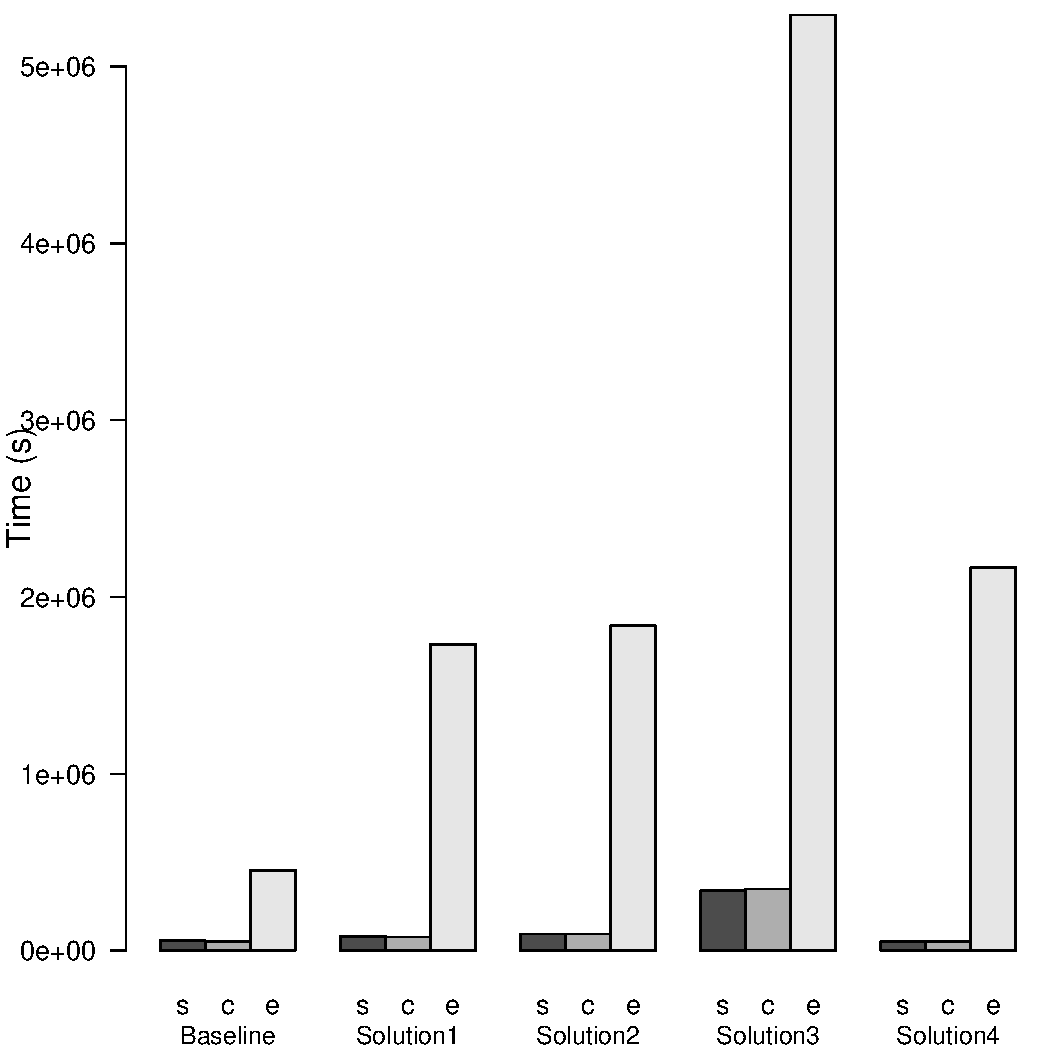
\includegraphics[width=\Width]{figure/result/barplot-insert-rt.pdf}}
			\subfigure[Throughput]
			{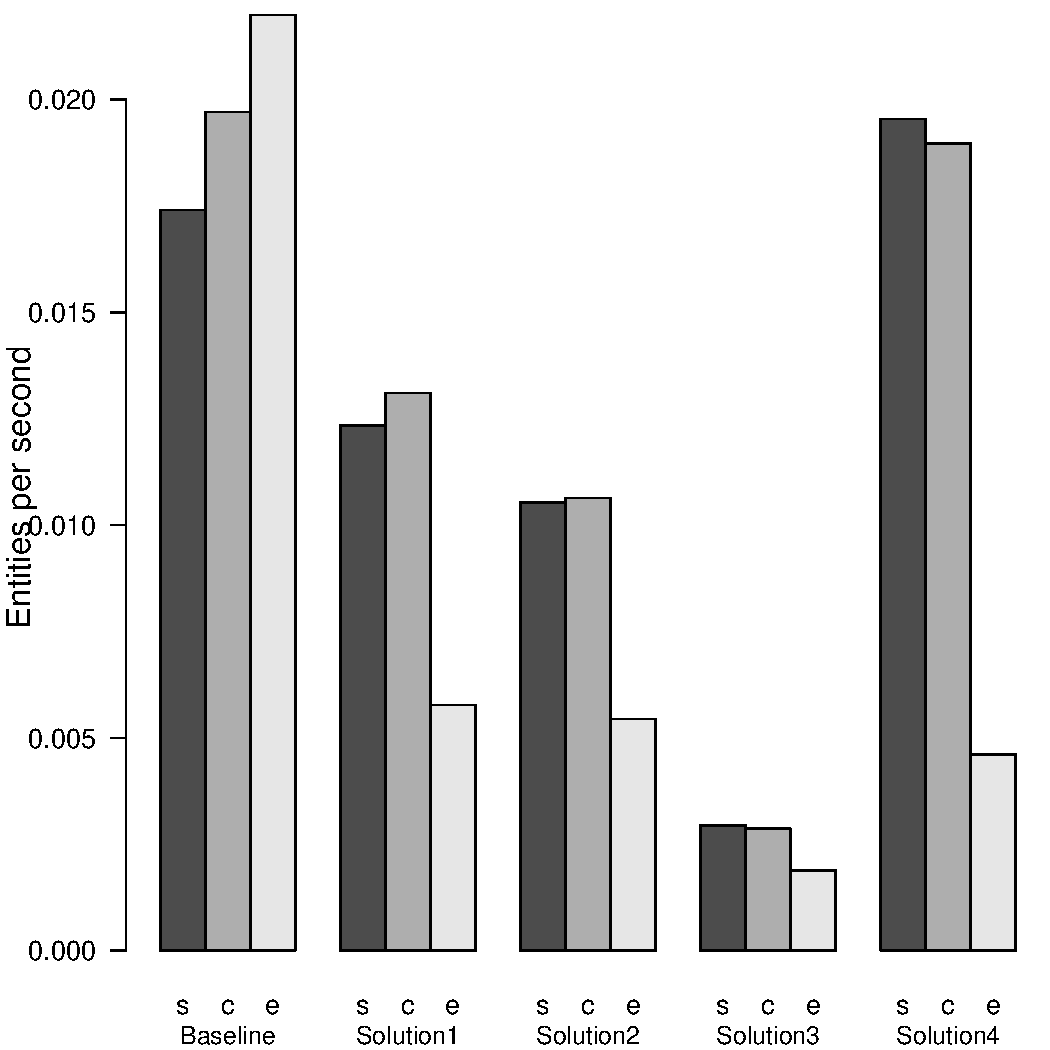
\includegraphics[width=\Width]{figure/result/barplot-insert-tp.pdf}}
			\caption{Performance of \texttt{insert}}\label{f:rd:insert}
		\end{figure}
		 
	\begin{figure}[c]
		\centering
		\subfigure[Response time]
		{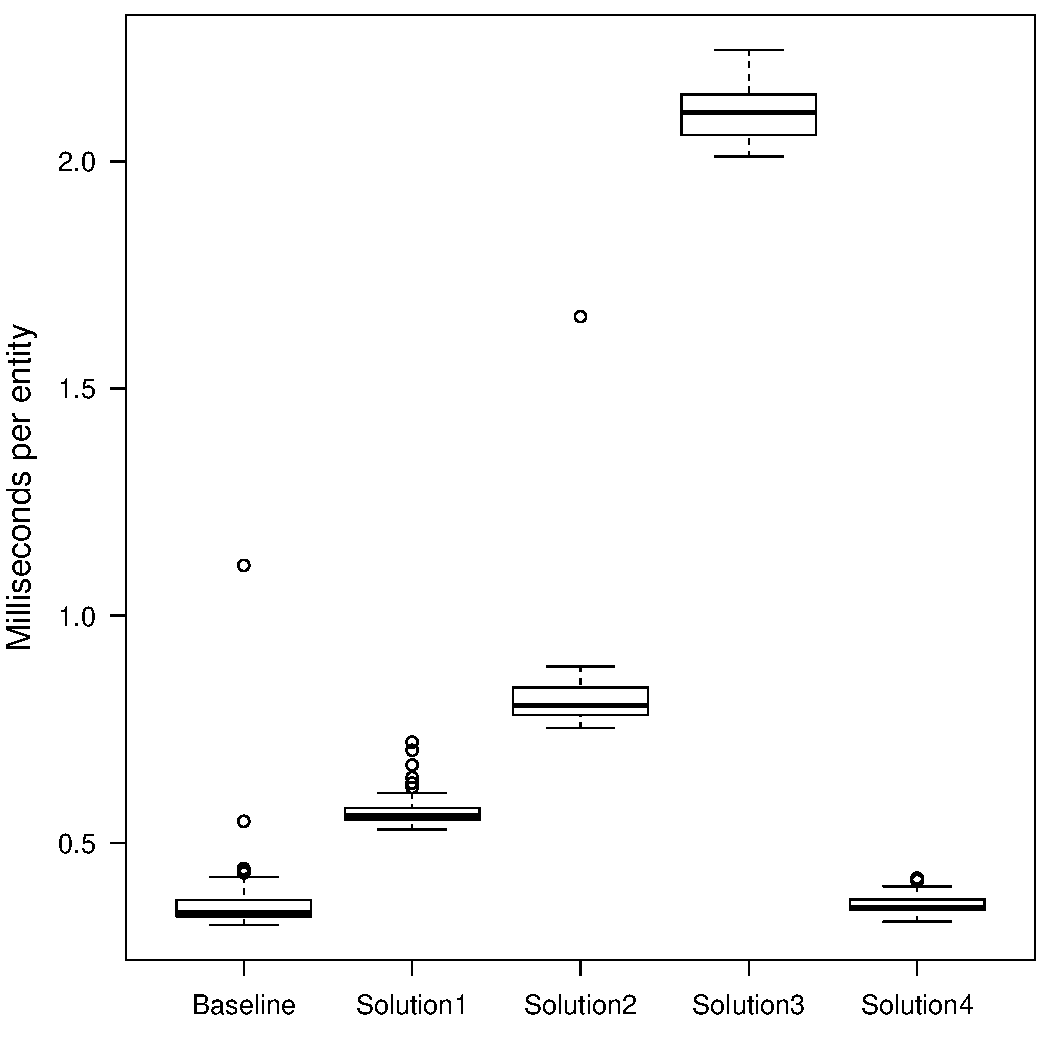
\includegraphics[width=\Width]{figure/result/boxplot-insert_student-rt.pdf}}
		\subfigure[Throughput]
		{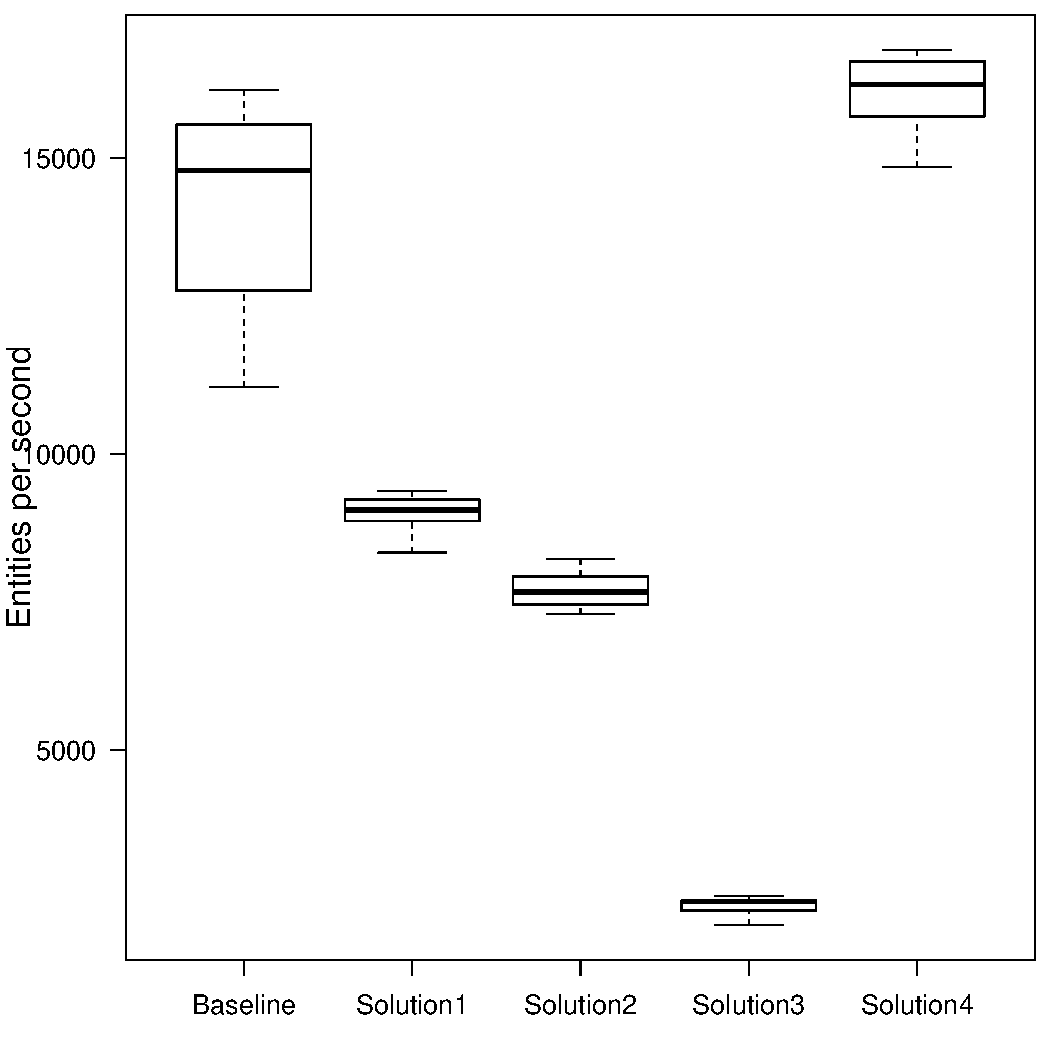
\includegraphics[width=\Width]{figure/result/boxplot-insert_student-tp.pdf}}
		\caption{Performance of \texttt{insert} students}
	\end{figure}
	

	\begin{figure}[c]
		\centering
		\subfigure[Response time]
		{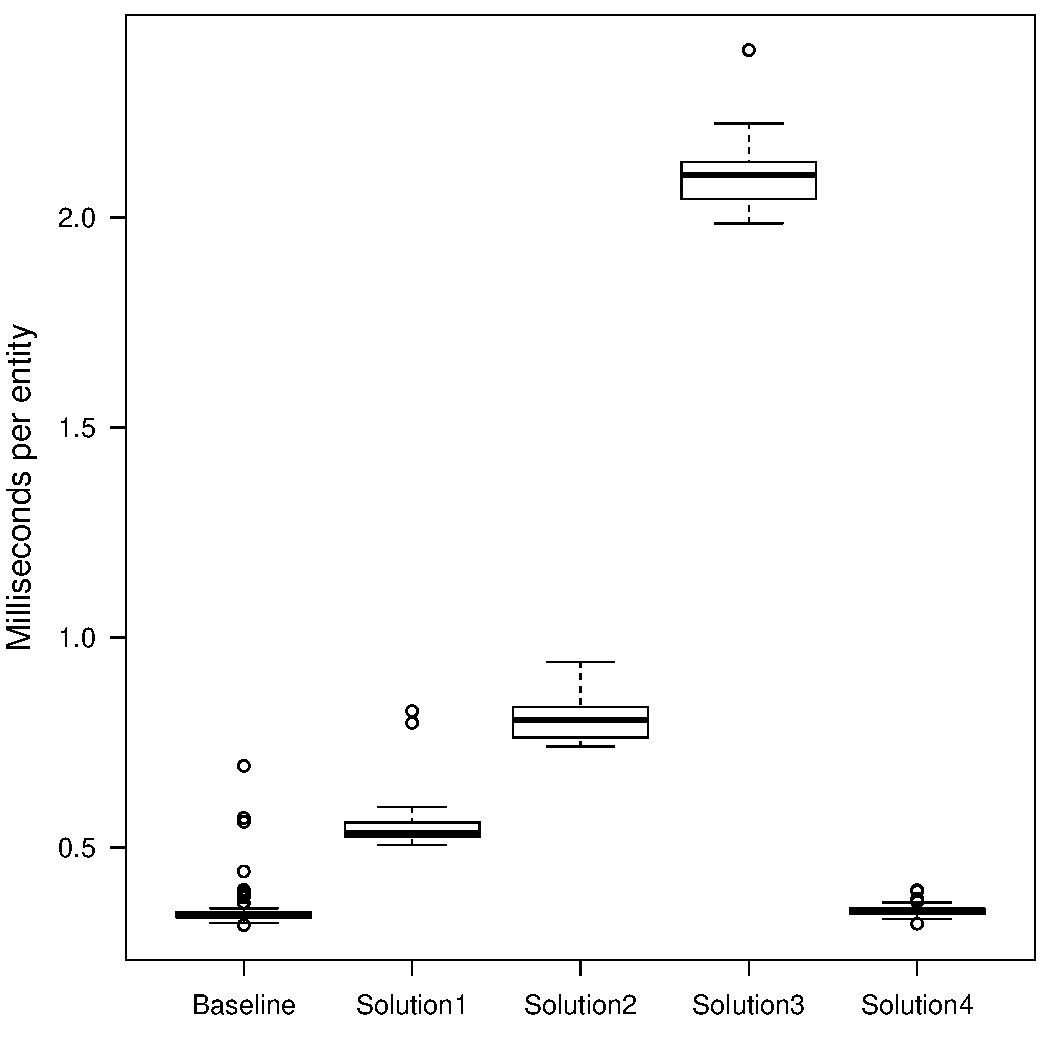
\includegraphics[width=\Width]{figure/result/boxplot-insert_course-rt.pdf}}
		\subfigure[Throughput]
		{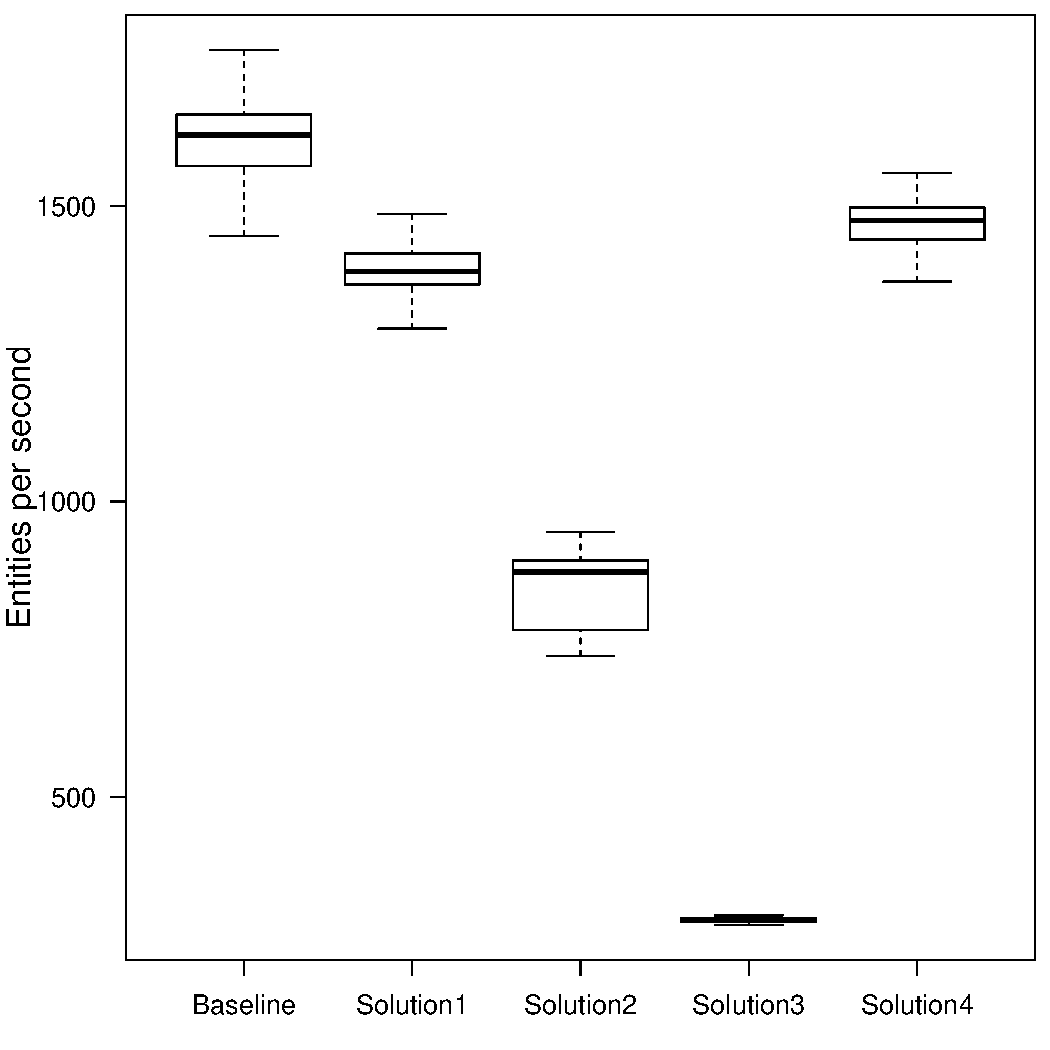
\includegraphics[width=\Width]{figure/result/boxplot-insert_course-tp.pdf}}
		\caption{Performance of \texttt{insert} courses}
	\end{figure}
 
 
	\begin{figure}[c]
		\centering
		\subfigure[Response time]
		{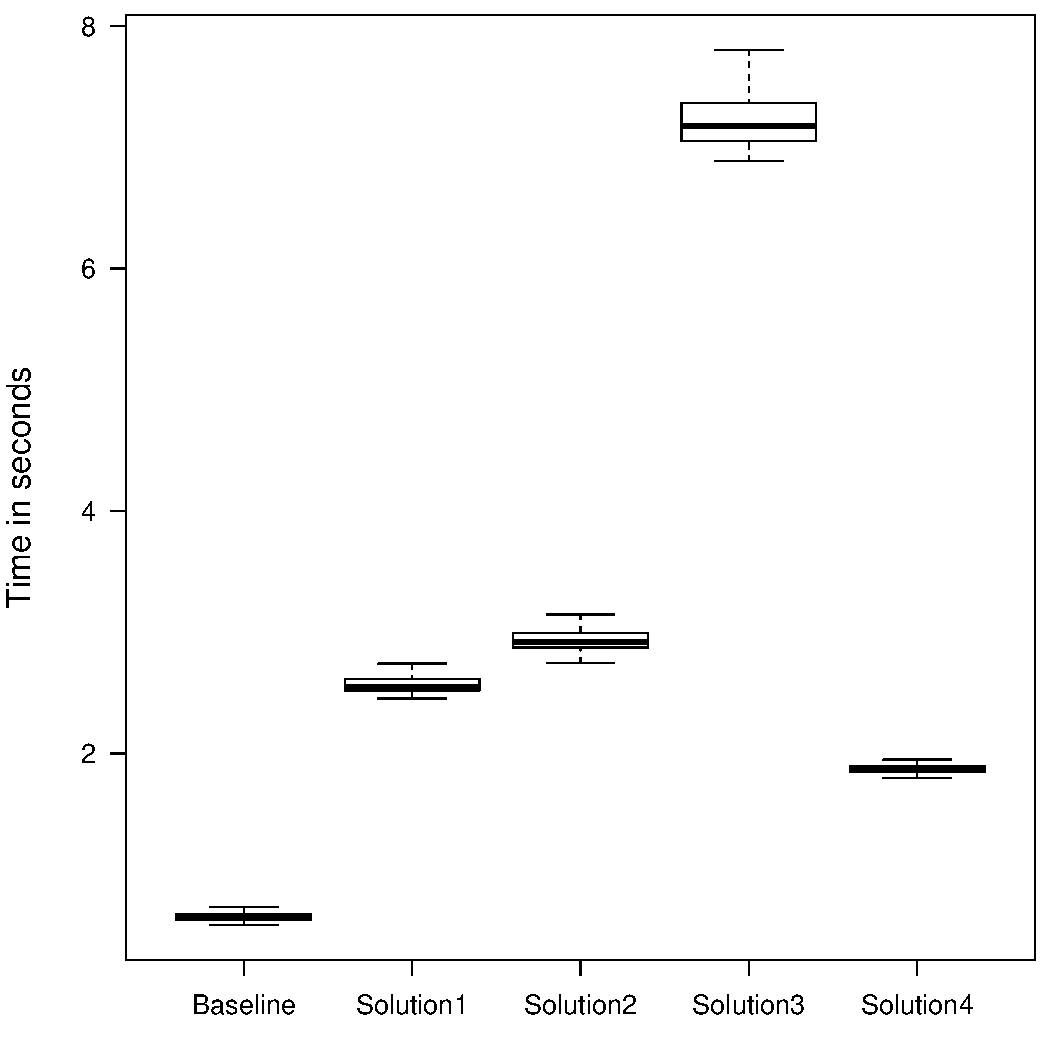
\includegraphics[width=\Width]{figure/result/boxplot-insert_enrolment-rt.pdf}}
		\subfigure[Throughput]
		{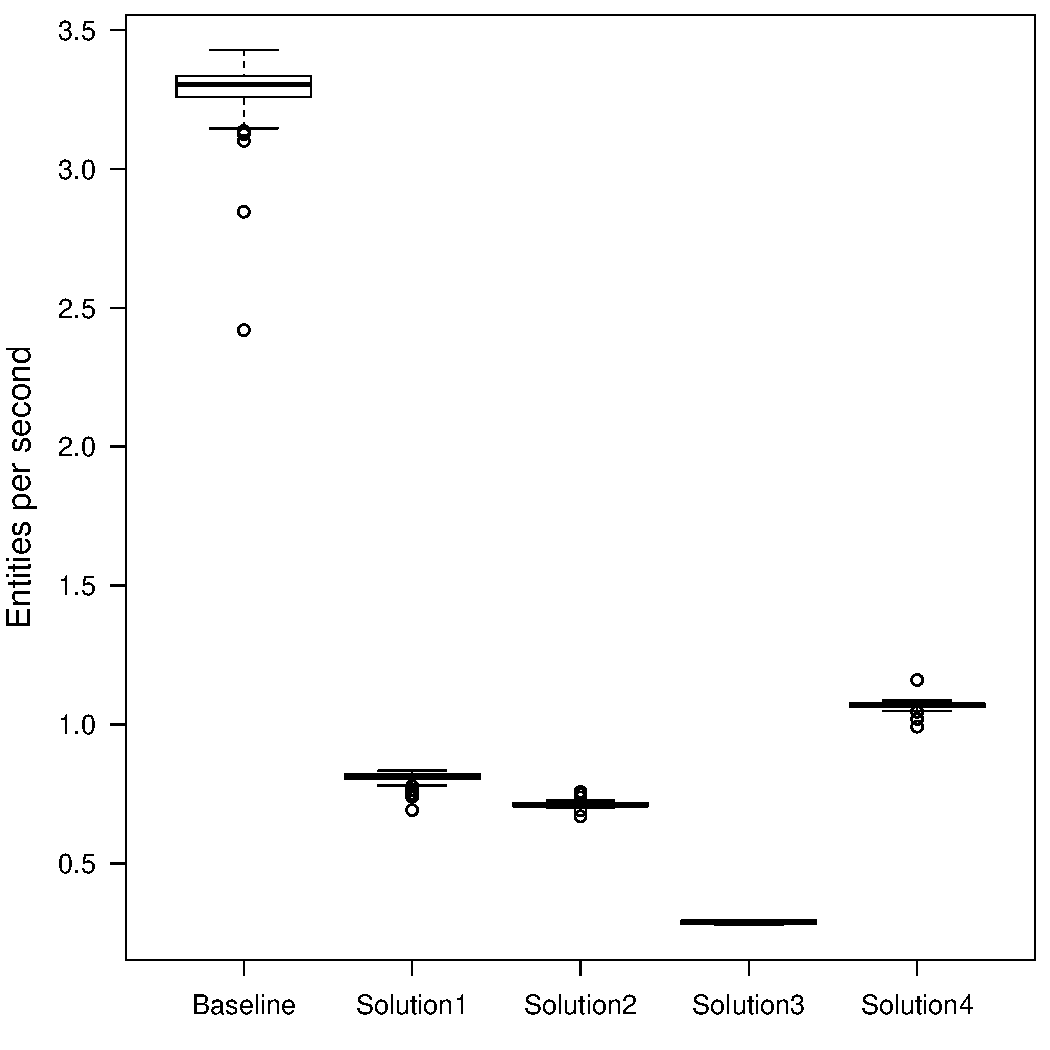
\includegraphics[width=\Width]{figure/result/boxplot-insert_enrolment-tp.pdf}}
		\caption{Performance of \texttt{insert} enrolments}
	\end{figure}
	
	
	
	
\chapter{Update}\label{apx:update}
\vfill
\newpage
		\begin{figure}[c]
		\centering
			\subfigure[Response time]
			{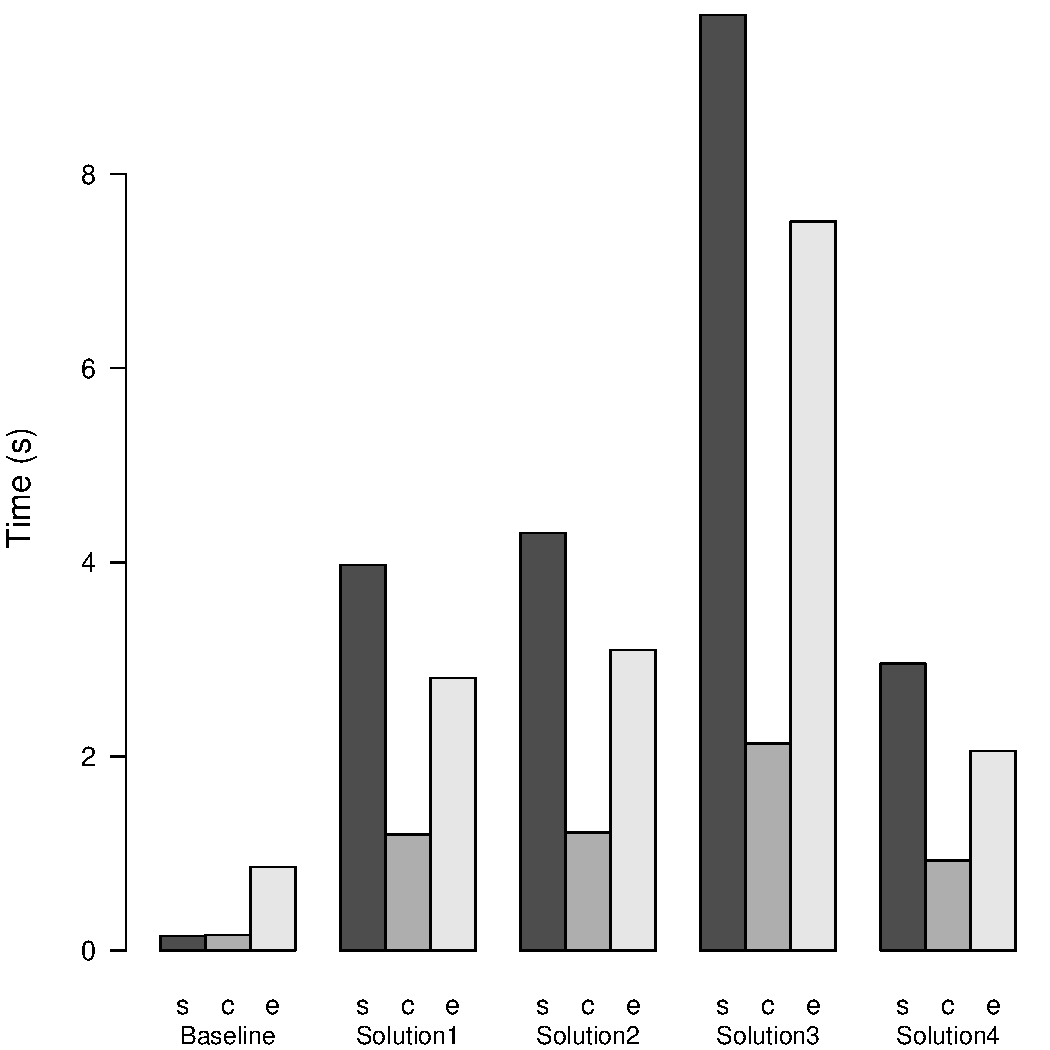
\includegraphics[width=\Width]{figure/result/barplot-update-rt.pdf}}
			\subfigure[Throughput]
			{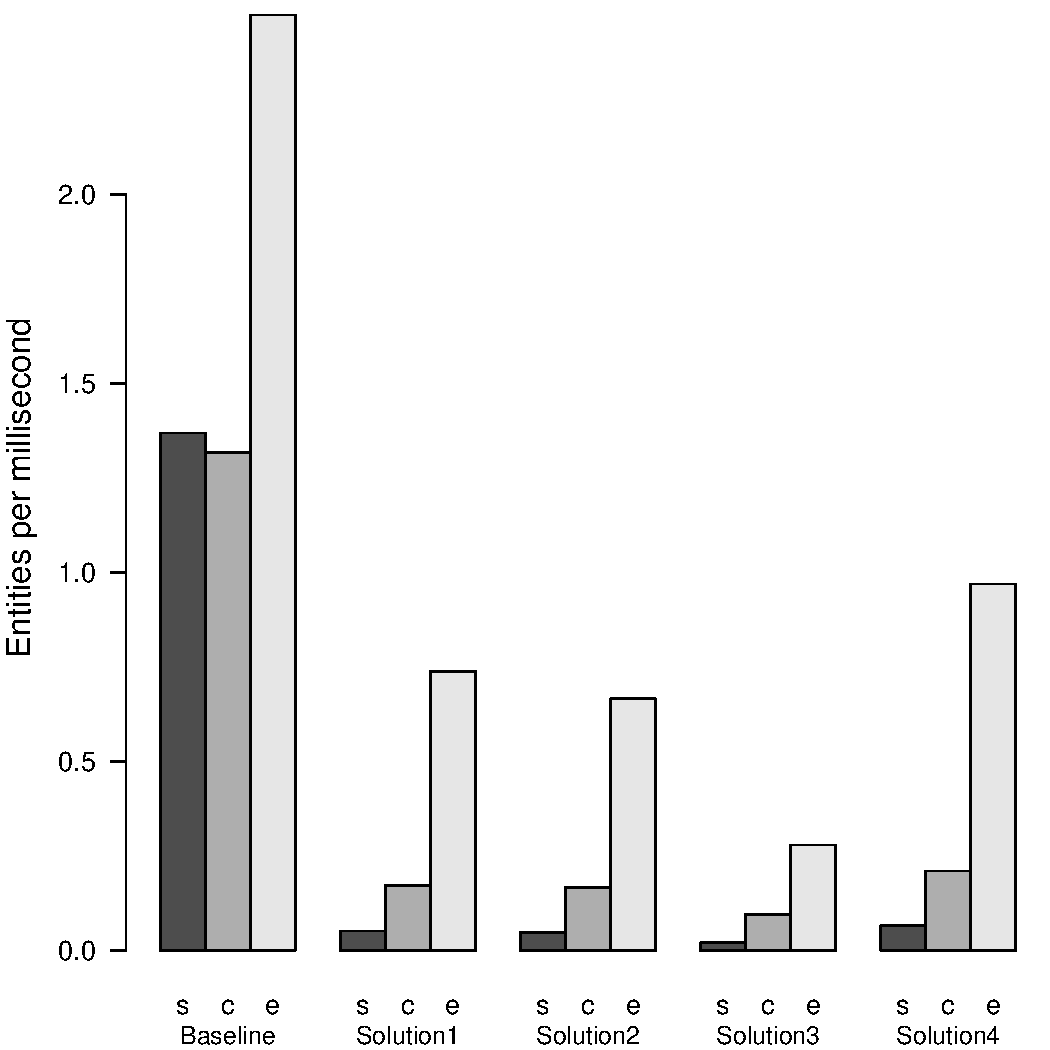
\includegraphics[width=\Width]{figure/result/barplot-update-tp.pdf}}
			\caption{Performance of \texttt{update}}\label{f:rd:update}
		\end{figure}
 
		
		
	\begin{figure}[c]
		\centering
		\subfigure[Response time]
		{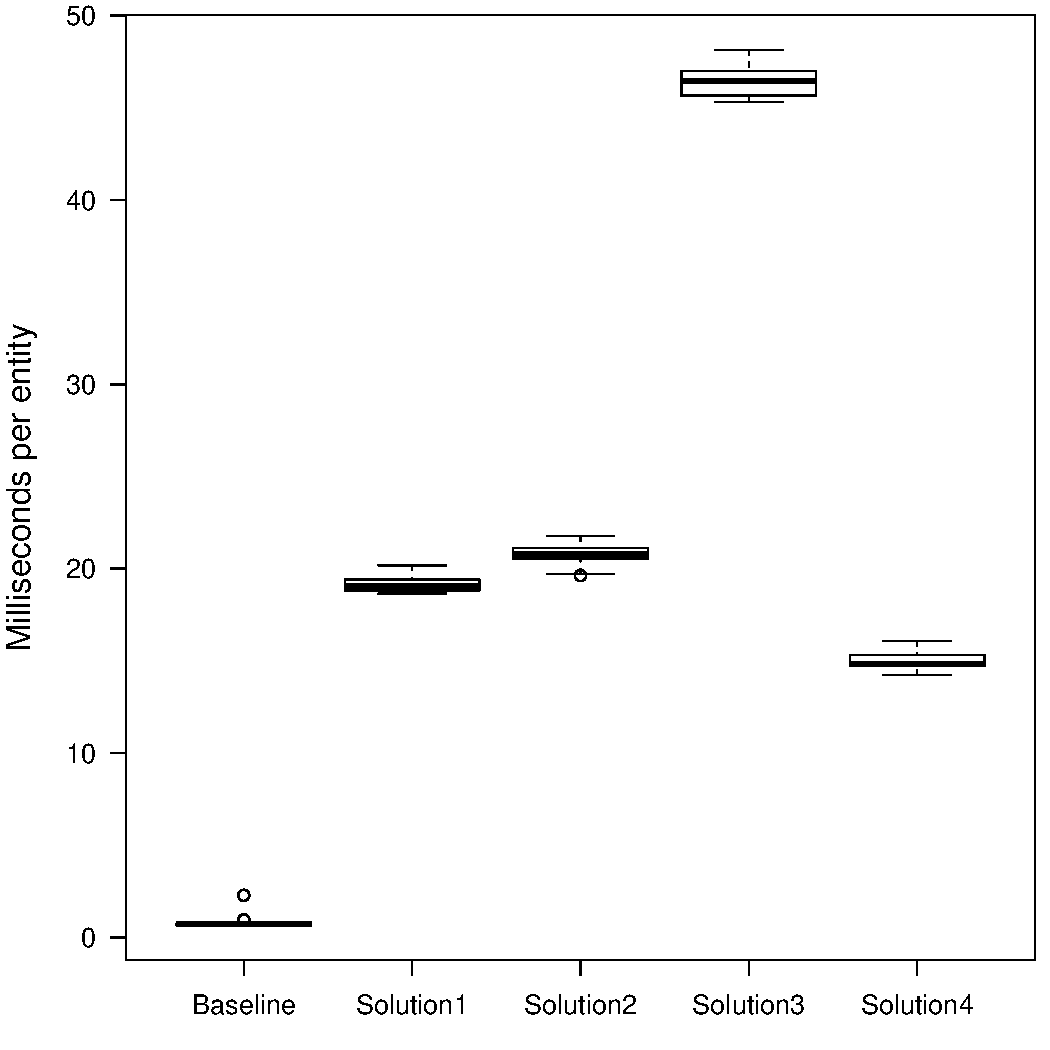
\includegraphics[width=\Width]{figure/result/boxplot-update_student-rt.pdf}}
		\subfigure[Throughput]
		{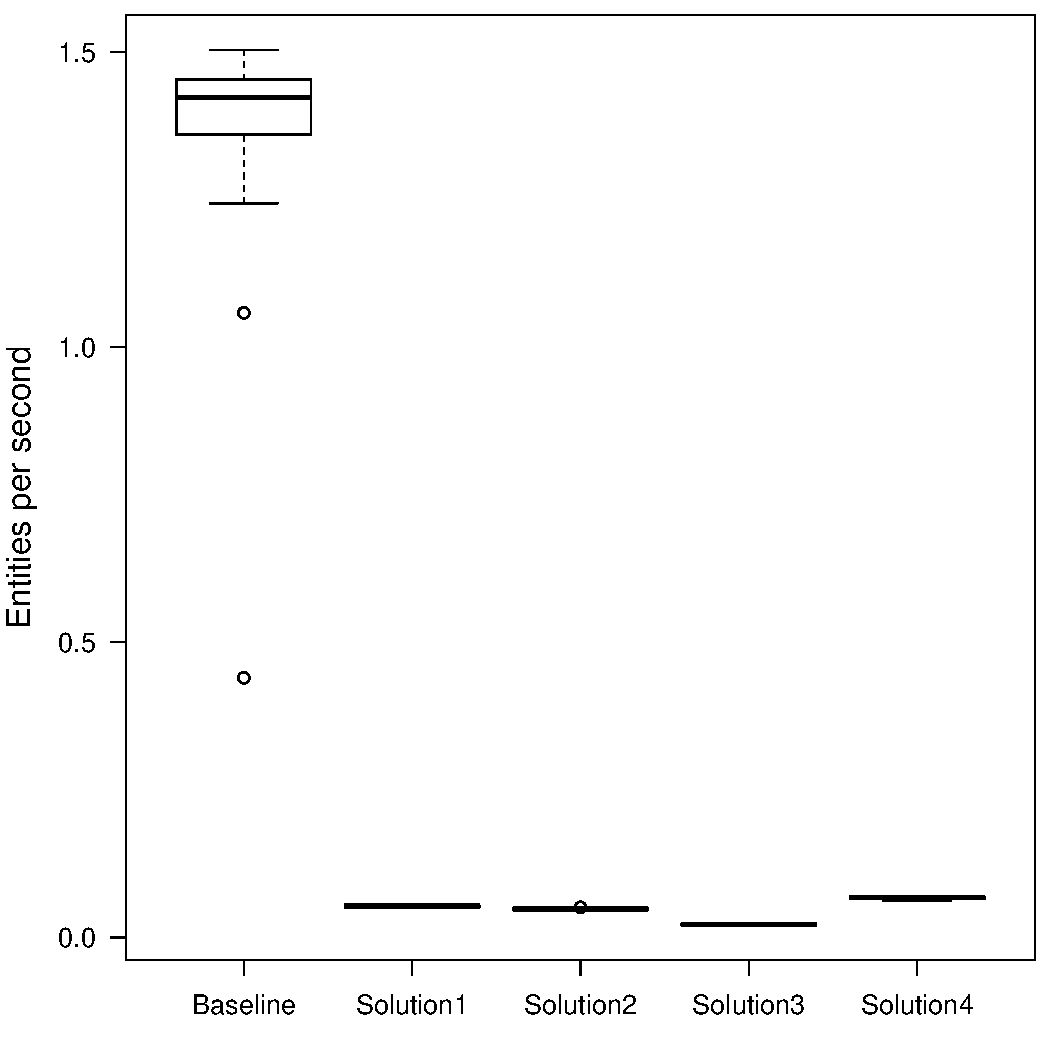
\includegraphics[width=\Width]{figure/result/boxplot-update_student-tp.pdf}}
		\caption{Performance of \texttt{update} students}
	\end{figure}
	

	\begin{figure}[c]
		\centering
		\subfigure[Response time]
		{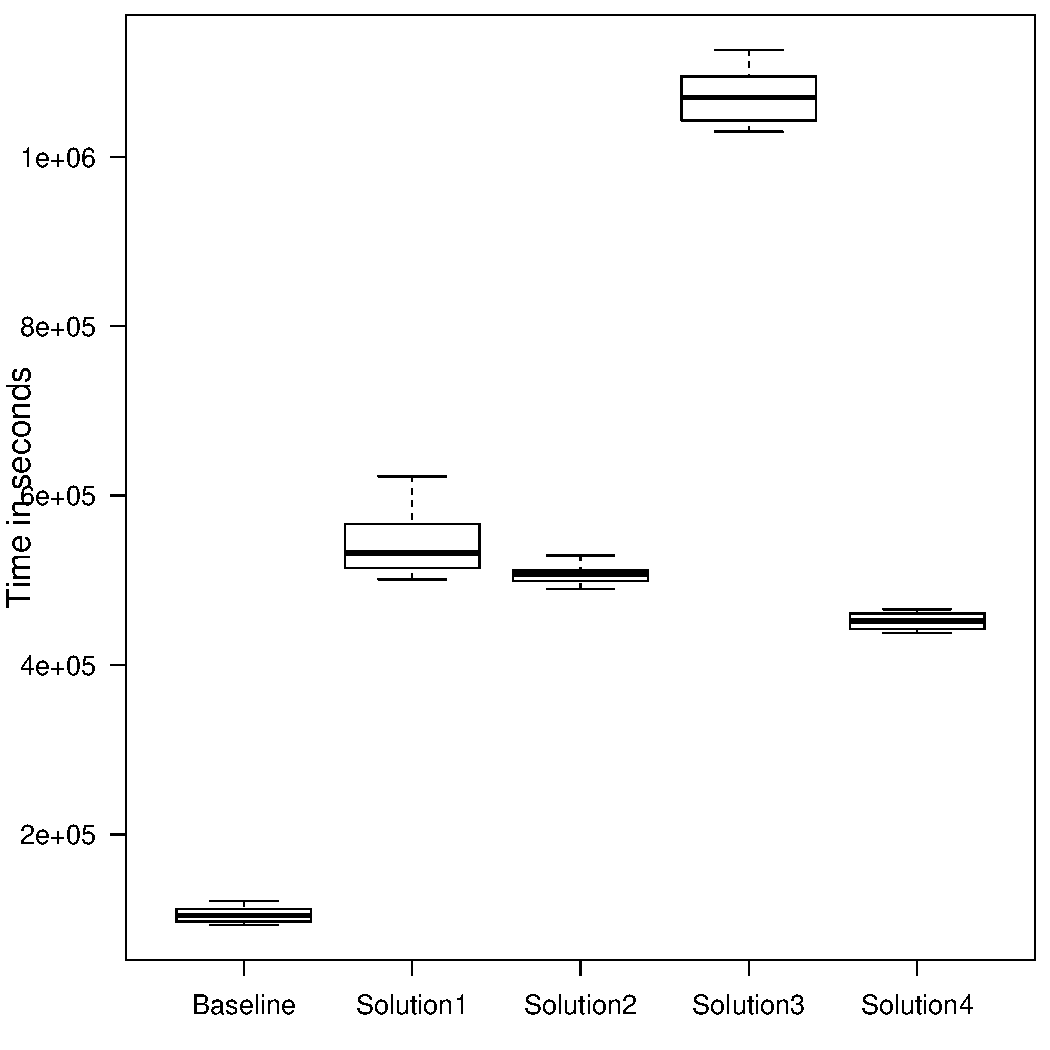
\includegraphics[width=\Width]{figure/result/boxplot-update_course-rt.pdf}}
		\subfigure[Throughput]
		{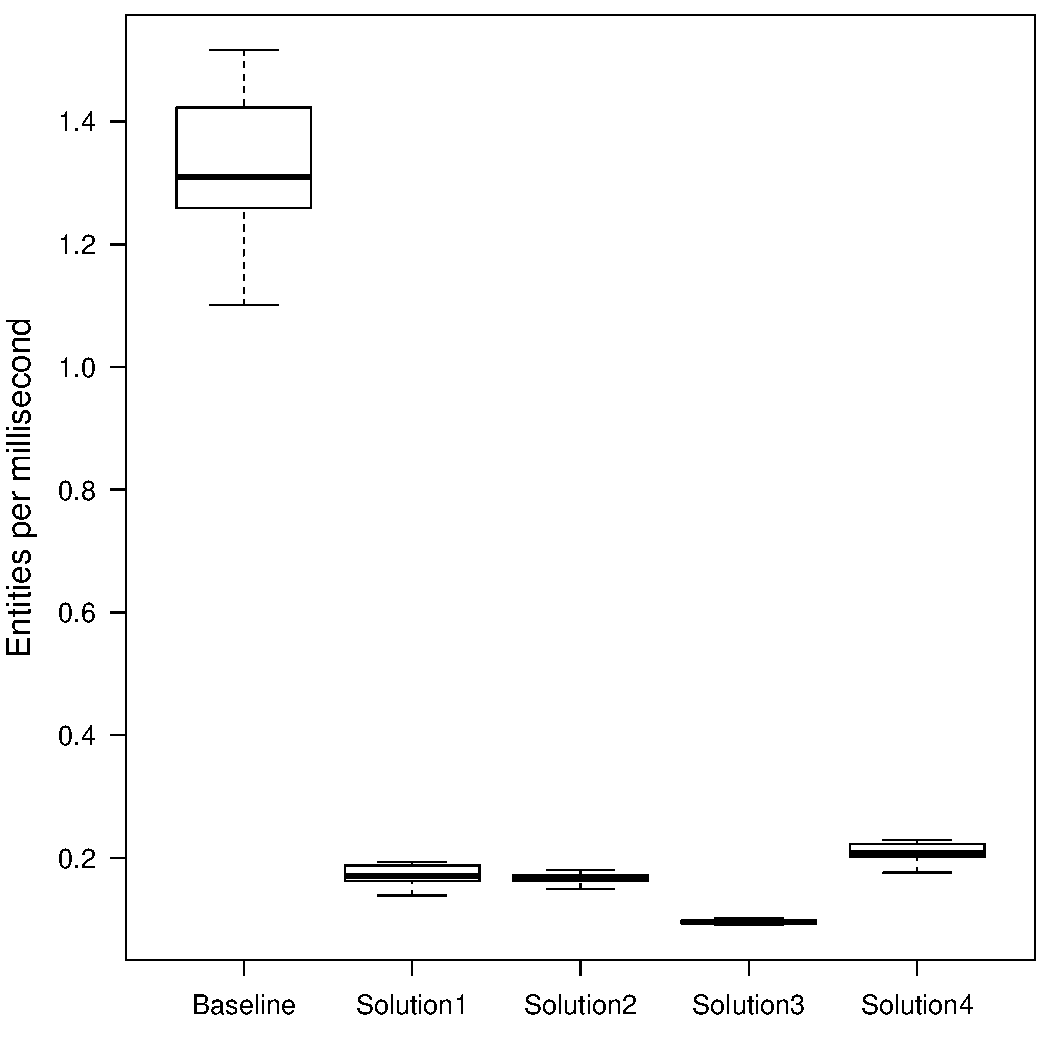
\includegraphics[width=\Width]{figure/result/boxplot-update_course-tp.pdf}}
		\caption{Performance of \texttt{update} courses}
	\end{figure}
 
 
	\begin{figure}[c]
		\centering
		\subfigure[Response time]
		{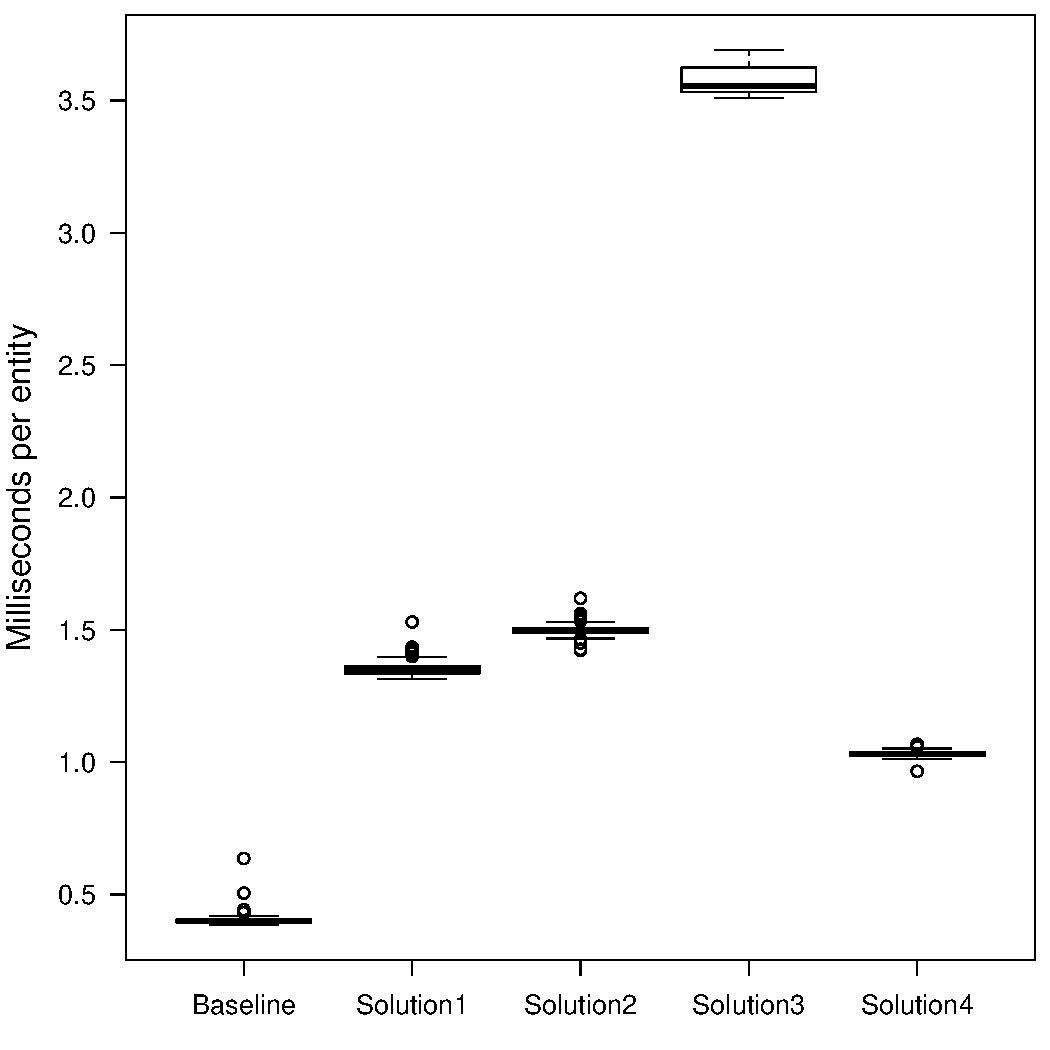
\includegraphics[width=\Width]{figure/result/boxplot-update_enrolment-rt.pdf}}
		\subfigure[Throughput]
		{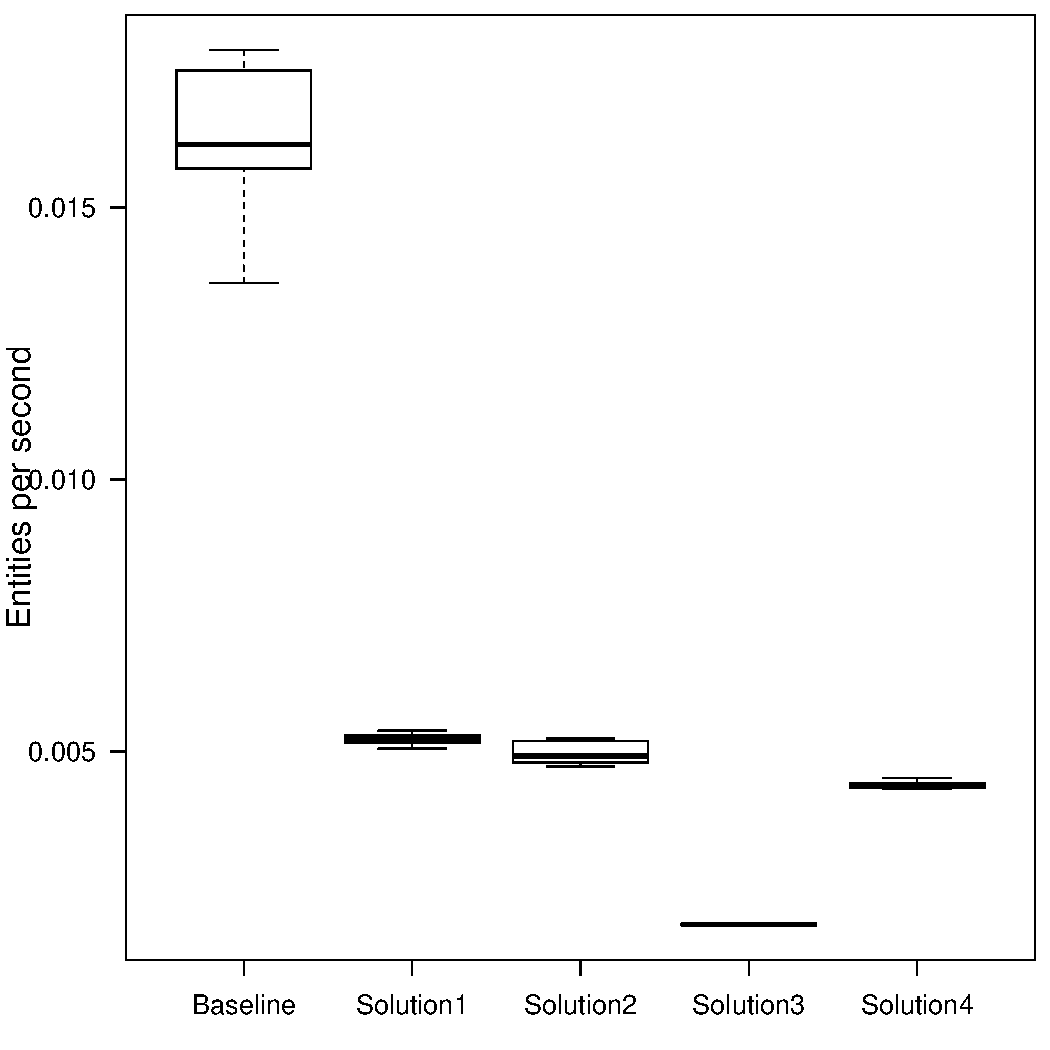
\includegraphics[width=\Width]{figure/result/boxplot-update_enrolment-tp.pdf}}
		\caption{Performance of \texttt{update} enrolments}
	\end{figure}	
	
	
	
	
\chapter{Delete}\label{apx:delete}
\vfill
\newpage
\begin{figure}[c]
		\centering
			\subfigure[Response time]
			{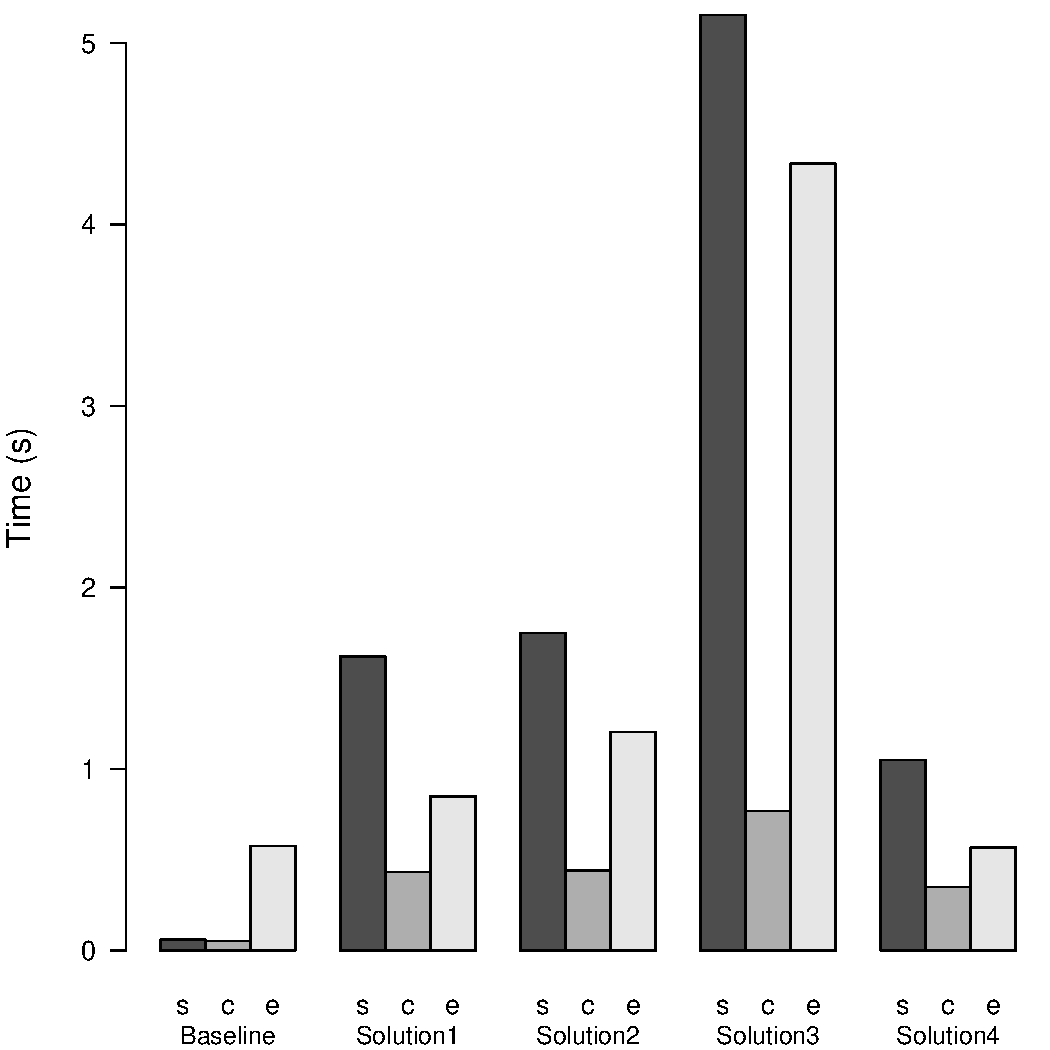
\includegraphics[width=\Width]{figure/result/barplot-delete-rt.pdf}}
			\subfigure[Throughput]
			{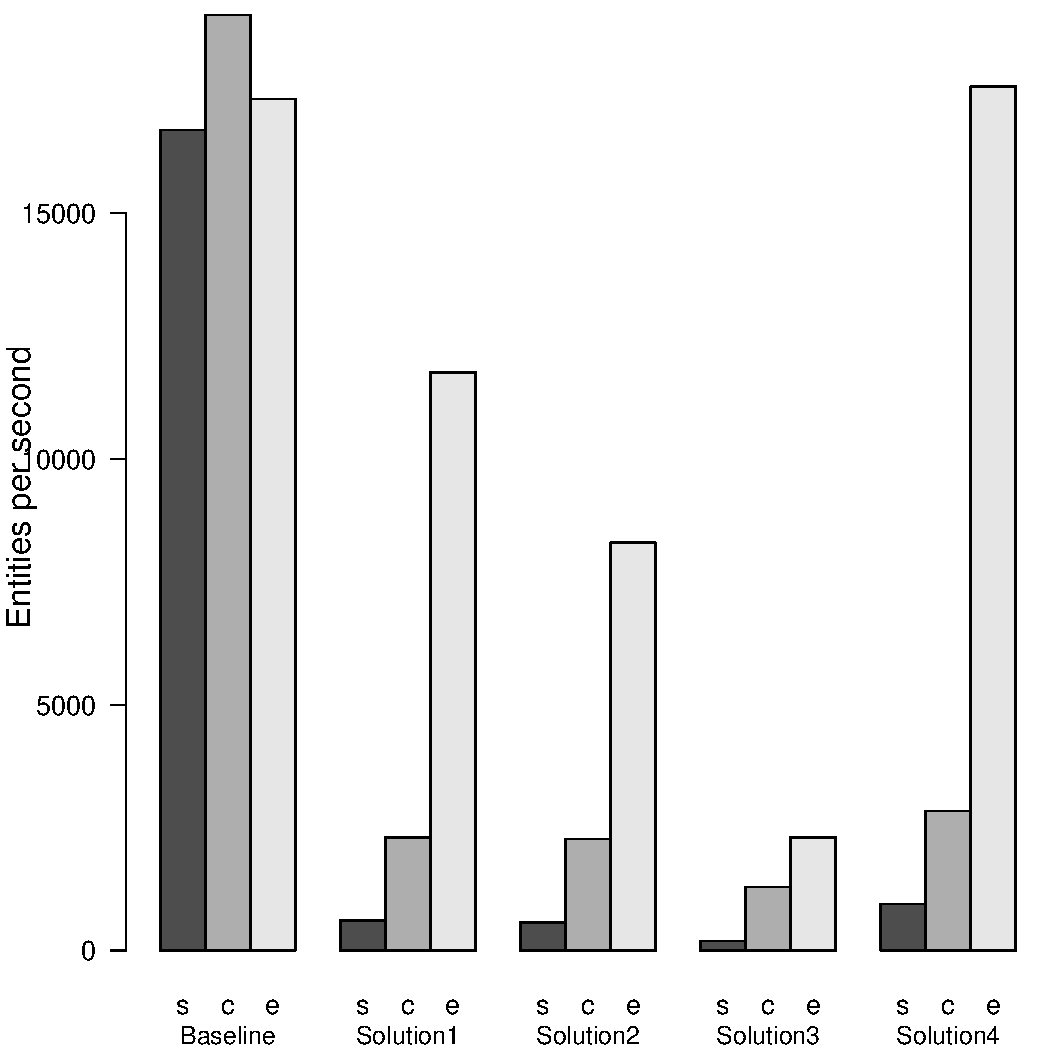
\includegraphics[width=\Width]{figure/result/barplot-delete-tp.pdf}}
			\caption{Performance of \texttt{delete}}\label{f:rd:delete}
		\end{figure}
		
	\begin{figure}[c]
		\centering
		\subfigure[Response time]
		{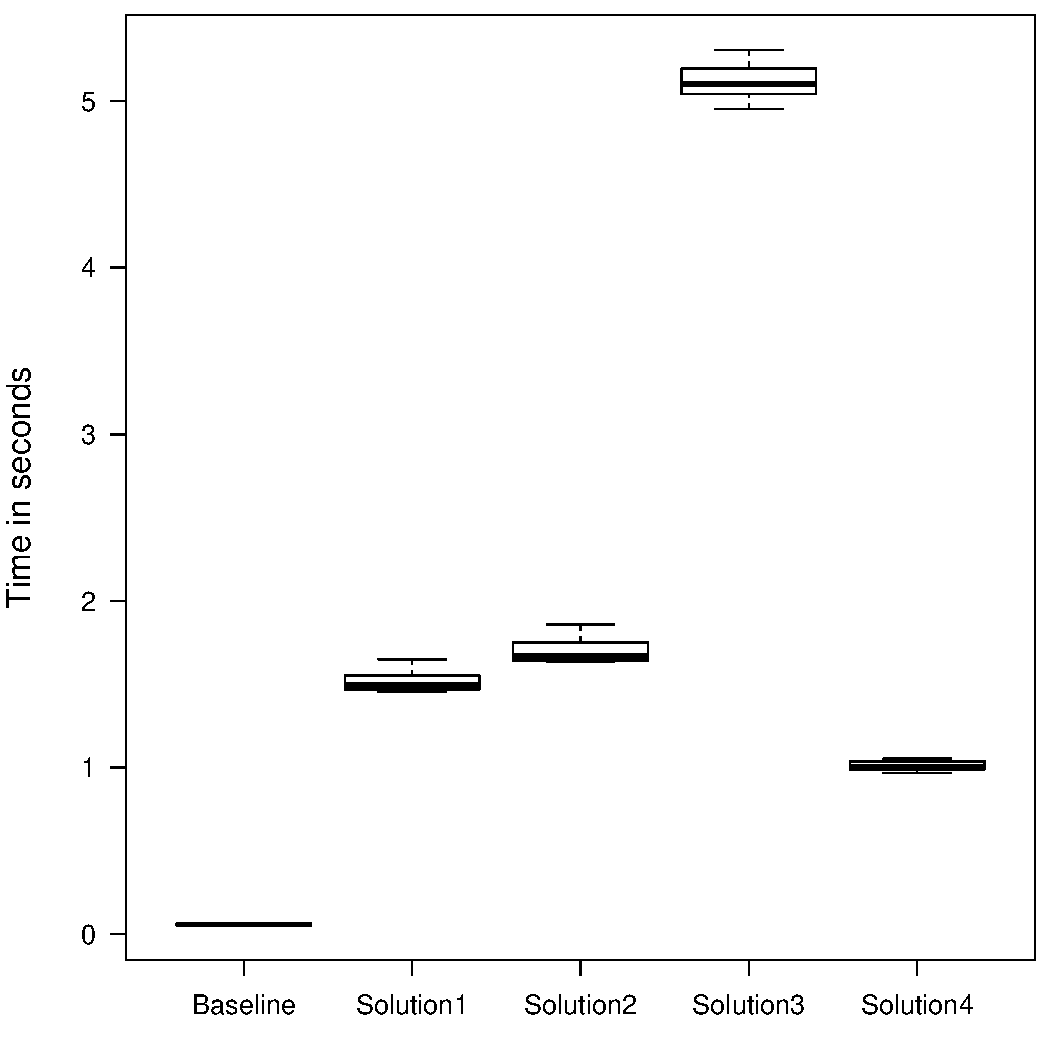
\includegraphics[width=\Width]{figure/result/boxplot-delete_student-rt.pdf}}
		\subfigure[Throughput]
		{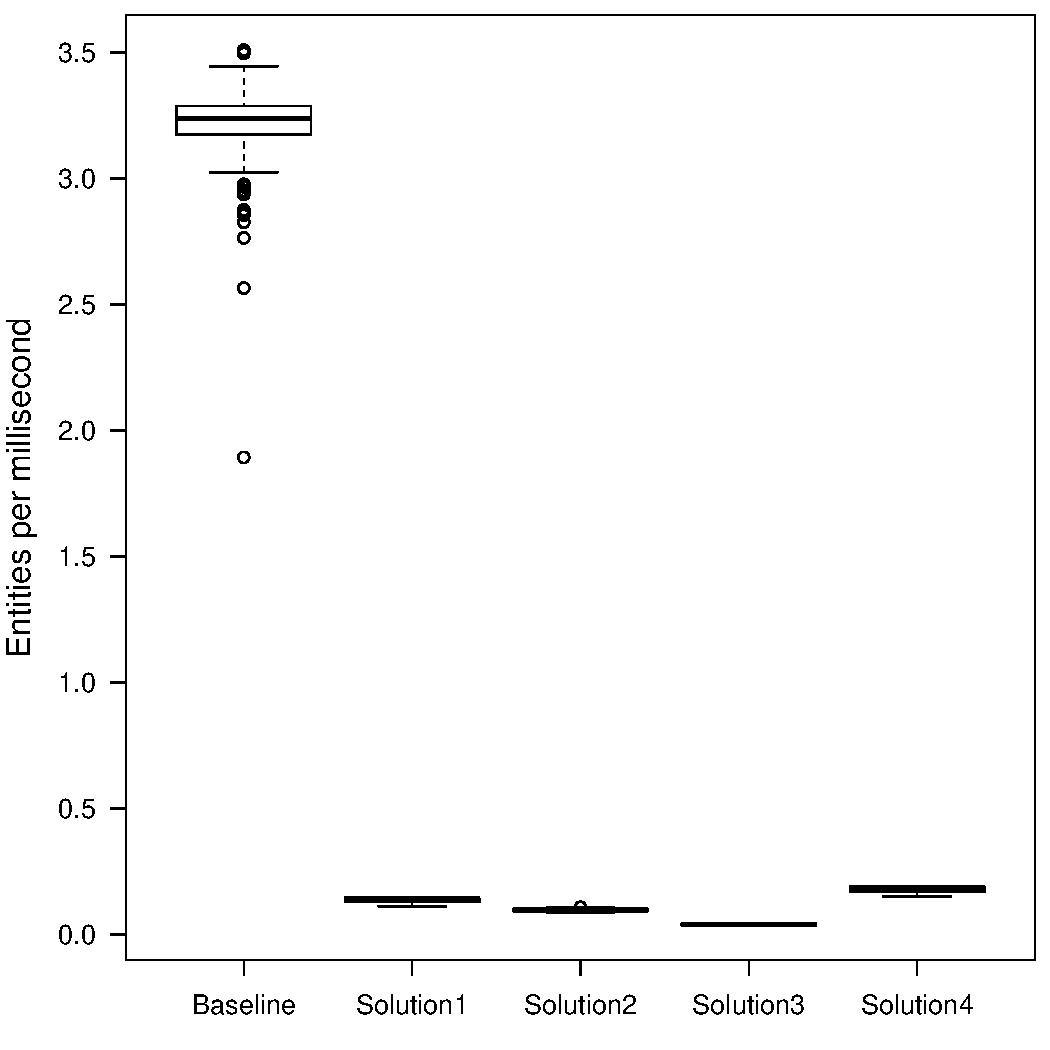
\includegraphics[width=\Width]{figure/result/boxplot-delete_student-tp.pdf}}
		\caption{Performance of \texttt{delete} students}
	\end{figure}
	

	\begin{figure}[c]
		\centering
		\subfigure[Response time]
		{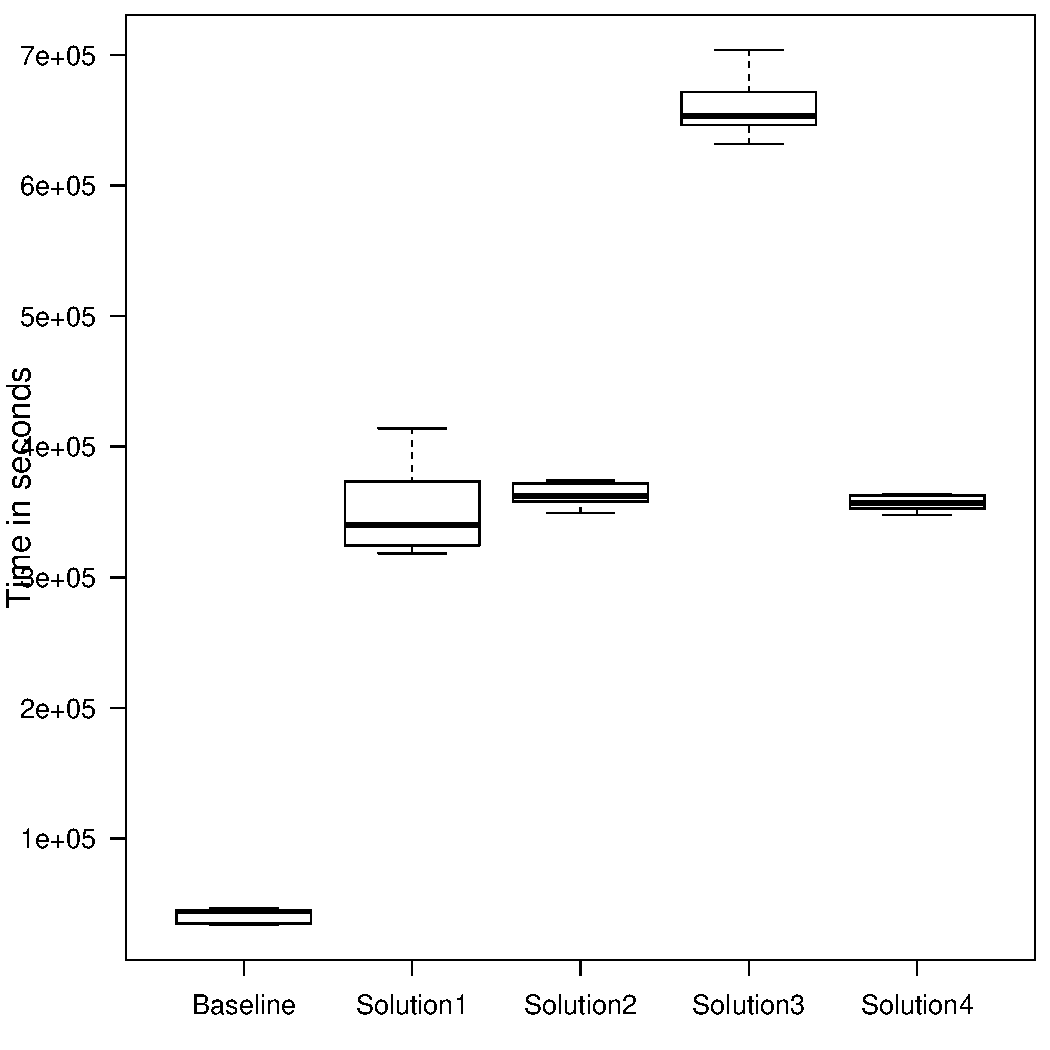
\includegraphics[width=\Width]{figure/result/boxplot-delete_course-rt.pdf}}
		\subfigure[Throughput]
		{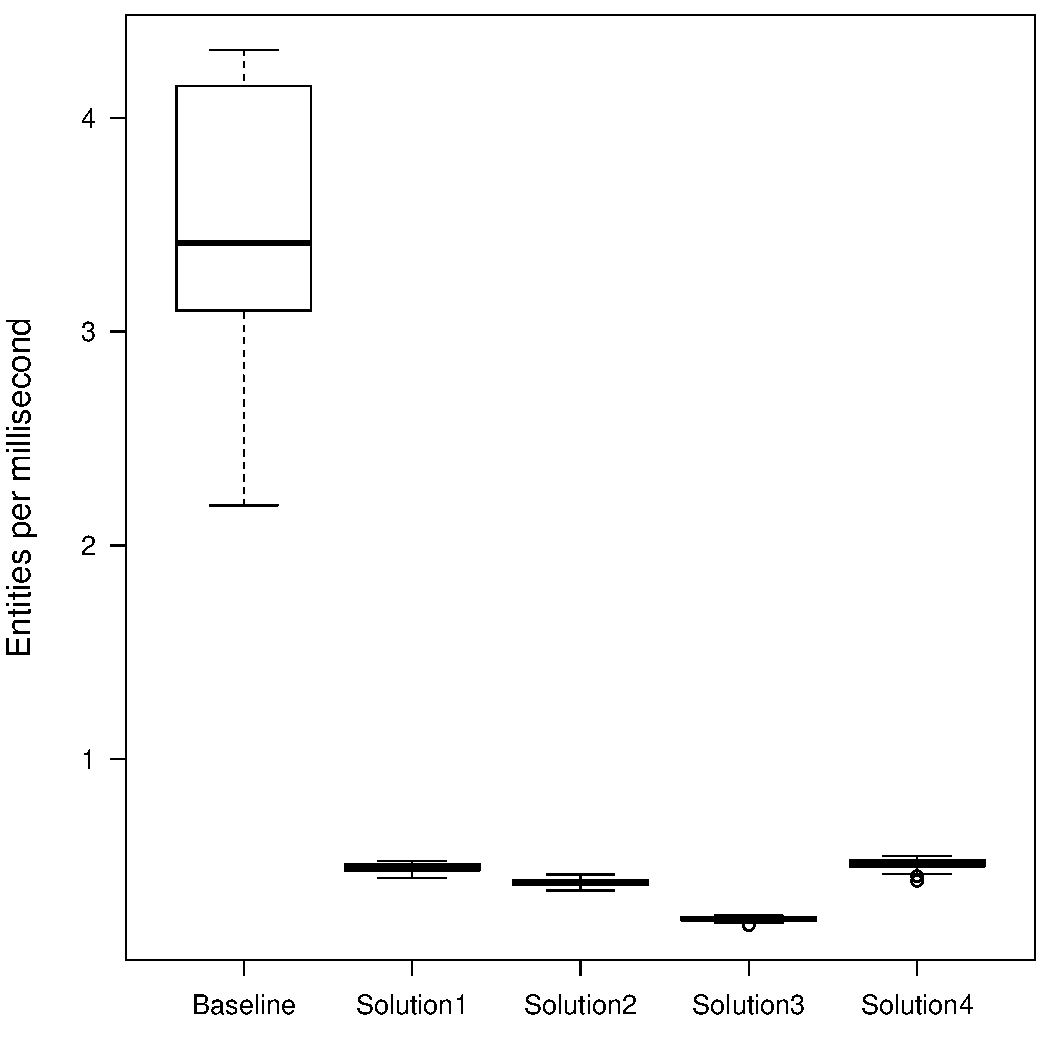
\includegraphics[width=\Width]{figure/result/boxplot-delete_course-tp.pdf}}
		\caption{Performance of \texttt{delete} courses}
	\end{figure}
 
 
	\begin{figure}[c]
		\centering
		\subfigure[Response time]
		{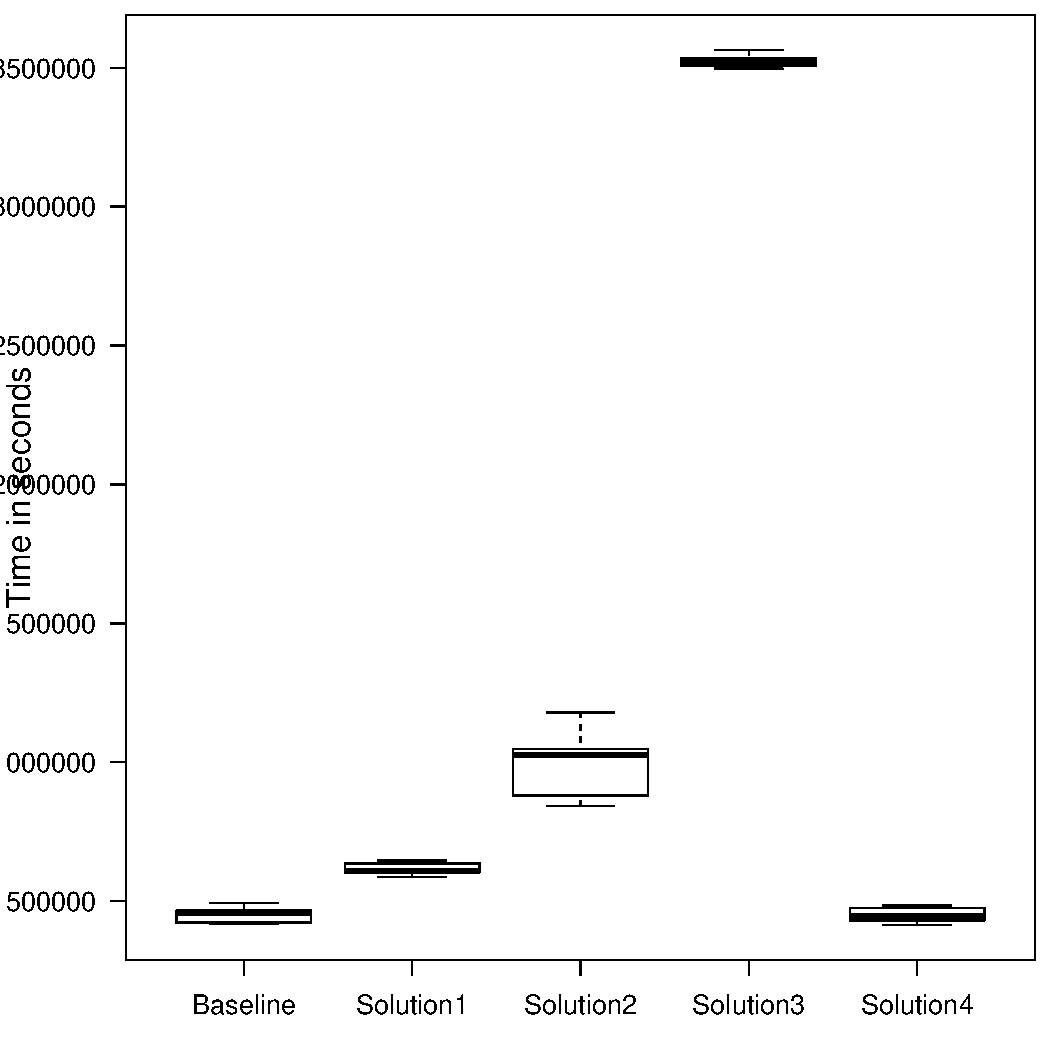
\includegraphics[width=\Width]{figure/result/boxplot-delete_enrolment-rt.pdf}}
		\subfigure[Throughput]
		{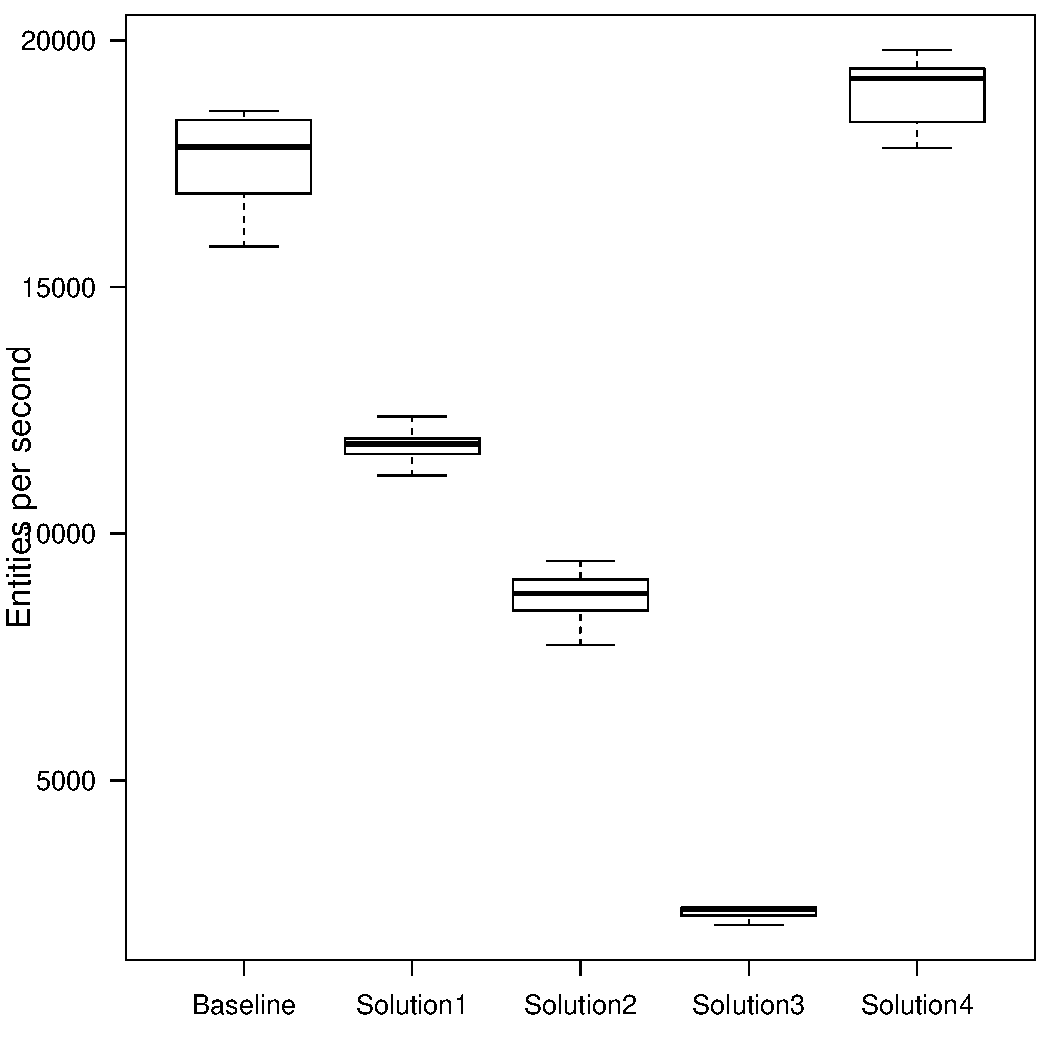
\includegraphics[width=\Width]{figure/result/boxplot-delete_enrolment-tp.pdf}}
		\caption{Performance of \texttt{delete} enrolments}
	\end{figure}